\documentclass[a4paper, 11pt]{article}
    \usepackage[fontset = windowsnew]{ctex}
    \usepackage{geometry}
        \geometry{left=2.54cm,right=2.54cm,top=3.18cm,bottom=3.18cm}
    \usepackage{amsmath}
    \usepackage{amsfonts}
    \usepackage{amssymb}
    \usepackage{siunitx}
    \usepackage{booktabs}
    \usepackage{longtable}
    \usepackage{graphicx}
    \usepackage{subfig}
    \usepackage{float}
    \usepackage{fancyvrb}
    \usepackage[unicode]{hyperref}
    \usepackage{xcolor}
    \usepackage{cite}
    
    \usepackage{listings}
    \lstset{
        %行号
        numbers=left,
        %背景框
        framexleftmargin=10mm,
        frame=none,
        %背景色
        %backgroundcolor=\color[rgb]{1,1,0.76},
        backgroundcolor=\color[RGB]{245,245,244},
        %样式
        basicstyle=\ttfamily,
        keywordstyle=\bf\color{blue},
        numberstyle=\color[RGB]{0,192,192},
        commentstyle=\it\color[RGB]{0,96,96},
        stringstyle=\rmfamily\slshape\color[RGB]{128,0,0},
        %显示空格
        showstringspaces=false
    }
    
    %%%%%% 设置字号 %%%%%%
    \newcommand{\chuhao}{\fontsize{42pt}{\baselineskip}\selectfont}
    \newcommand{\xiaochuhao}{\fontsize{36pt}{\baselineskip}\selectfont}
    \newcommand{\yihao}{\fontsize{28pt}{\baselineskip}\selectfont}
    \newcommand{\erhao}{\fontsize{21pt}{\baselineskip}\selectfont}
    \newcommand{\xiaoerhao}{\fontsize{18pt}{\baselineskip}\selectfont}
    \newcommand{\sanhao}{\fontsize{15.75pt}{\baselineskip}\selectfont}
    \newcommand{\sihao}{\fontsize{14pt}{\baselineskip}\selectfont}
    \newcommand{\xiaosihao}{\fontsize{12pt}{\baselineskip}\selectfont}
    \newcommand{\wuhao}{\fontsize{10.5pt}{\baselineskip}\selectfont}
    \newcommand{\xiaowuhao}{\fontsize{9pt}{\baselineskip}\selectfont}
    \newcommand{\liuhao}{\fontsize{7.875pt}{\baselineskip}\selectfont}
    \newcommand{\qihao}{\fontsize{5.25pt}{\baselineskip}\selectfont}

\begin{document}
%%%% 定理类环境的定义 %%%%
\newtheorem{example}{例}             % 整体编号
\newtheorem{algorithm}{算法}
\newtheorem{theorem}{定理}[section]  % 按 section 编号
\newtheorem{definition}{定义}
\newtheorem{axiom}{公理}
\newtheorem{property}{性质}
\newtheorem{proposition}{命题}
\newtheorem{lemma}{引理}
\newtheorem{corollary}{推论}
\newtheorem{remark}{注解}
\newtheorem{condition}{条件}
\newtheorem{conclusion}{结论}
\newtheorem{assumption}{假设}
\newtheorem{problem}{问题}
%%%% 重定义 %%%%
\renewcommand{\contentsname}{目录}  % 将Contents改为目录
\renewcommand{\abstractname}{摘要}  % 将Abstract改为摘要
\renewcommand{\refname}{参考文献}   % 将References改为参考文献
\renewcommand{\indexname}{索引}
\renewcommand{\figurename}{图}
\renewcommand{\tablename}{表}
\renewcommand{\appendixname}{附录}

    \title{\textbf{AVL树$\rightarrow$红黑树问题}\\\xiaosihao \emph{《现代操作系统》实验报告}}
    \author{王晗\\(2013011076)}
    \date{\today}
    \maketitle
    %\tableofcontents
    %\newpage

    \section{实验内容}
        在Windows的虚拟内存管理中,将VAD组织成AVL树。VAD树是一种平衡二叉树。红黑树也是一种自平衡二叉查找树,在Linux 2.6及其以后版本的内核中,采用红黑树来维护内存块。

        请尝试参考Linux源代码将WRK源代码中的VAD树由AVL树替换成红黑树。

    \section{实验环境搭建}
        实验使用\texttt{VirtualBox 5.0.8}作为虚拟机控制台,安装\texttt{Windows Server 2003 SP1}用于内核的调试。配置虚拟机串口,连接到命名管道:$\mathtt{\backslash\backslash.pipe\backslash debugger}$。将编译后的内核程序\texttt{wrkx86.exe}和硬件抽象层动态链接库\texttt{halacpim.dll}放置在$\mathtt{C:\backslash Windows\backslash system32}$ 下,并向\texttt{boot.ini}中添加启动项:
\begin{lstlisting}
multi(0)disk(0)rdisk(0)partition(1)\WINDOWS="Windows Server 2003, 
    WRK" /kernel=wrkx86.exe /hal=halacpim.dll
multi(0)disk(0)rdisk(0)partition(1)\WINDOWS="Windows Server 2003, 
    DEBUG" /kernel=wrkx86.exe /hal=halacpim.dll /debug
    /debugport=com1 /baudrate=115200
\end{lstlisting}
        
        在宿主机上安装\texttt{WinDbg},配置\texttt{Kernel Debugger}连接到相同的命名管道$\backslash\backslash.pipe\backslash debugger$进行双机调试。为了方便调试,还可以安装微软提供的
        \texttt{Windows Server 2003}符号集\\
        \texttt{Windows2003\_sp1.x86.fre.rtm.symbols}。
        
        实验中还需要\texttt{Windows Research Kernel(WRK)}和\texttt{Linux Kernel}源代码,其中\texttt{Linux Kernel}选择Long-term版本\texttt{linux-2.6.32.68}。
        
    \section{AVL树与红黑树}
        \subsection{AVL树简介}
        
        \subsection{红黑树简介}
        
        \subsection{Linux中的红黑树实现}
            \texttt{Linux Kernel}中的红黑树头文件和源文件分别位于 \\
            $\mathtt{linux-2.6.32.68\backslash include \backslash linux \backslash rbtree.h}$和 \\
            $\mathtt{linux-2.6.32.68 \backslash lib \backslash rbtree.c}$。
            
            根据开源文档\texttt{rbtree.txt}\cite{rbtreetxt}中的介绍,对\texttt{Linux Kernel}中的红黑树进行修改,并通过整数的插入删除进行测试。
            
            在这一过程中,需要删除上述文件中\texttt{Linux Kernel}头文件的引用和\texttt{EXPORT\_SYMBOL}宏,并补充部分宏定义,还需要完成自己的查找、插入、删除、遍历函数\footnote{代码见附件$\mathtt{codes\backslash rbtree\_test\backslash}$。}。需要注意的是,\texttt{Linux Kernel} 中的红黑树节点采用了32 位对齐,因此节点地址的低2位一定为0,因此每个节点可以使用双亲节点指针的低2位来记录其颜色。在\texttt{GCC}中,32位对齐可以使用预编译指令
\begin{lstlisting}[language={C}]
__attribute__((aligned(sizeof(long))))
\end{lstlisting}
            而在\texttt{Visual Studio}中等价的预编译指令为
\begin{lstlisting}[language={C}]
#pragma pack(4)
\end{lstlisting}
            
            使用修改后的红黑树完成整数的插入删除测试,结果如图\ref{fig:rbtreetest}所示。
            \begin{figure}[htb]
                \centering
                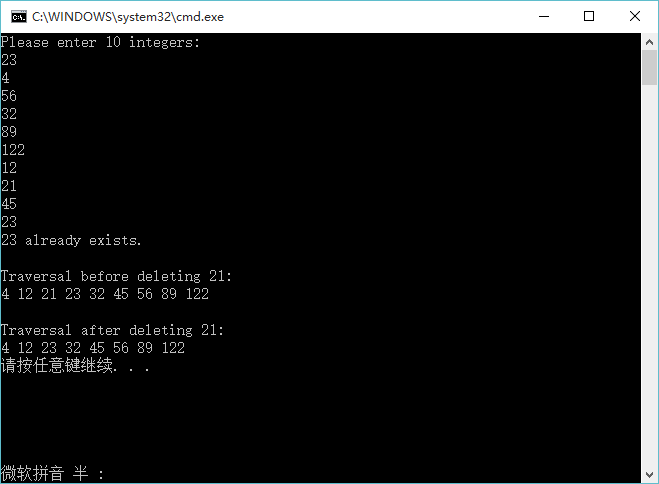
\includegraphics[width=15cm]{images/rbtreetest.png}
                \caption{红黑树插入删除测试}
                \label{fig:rbtreetest}
            \end{figure}
            
    \section{Windows进程地址空间的内存管理}
        \subsection{虚拟地址描述符与VAD树}
            
        \subsection{Windows中的AVL树实现}
            
        \subsection{Windows中的红黑树实现}
            
        
        
    \section{实验结果}
        将编译后的内核程序\texttt{wrkx86.exe}放入虚拟机,重新启动后选择\texttt{Windows Server 2003, WRK}启动项,可以正常启动系统。
        
        在宿主机中打开\texttt{WinDbg},进入内核调试,然后使用调试模式启动虚拟机,再启动一个程序(如记事本)。在\texttt{WinDbg}中使用\texttt{!process 0 0}命令查看所有进程,记录下\texttt{notepad.exe}的CID,然后使用\texttt{!process CID 1}命令查看\texttt{notepad.exe}的VAD树根节点地址,再使用\texttt{!vad addr}即可查看\texttt{notepad.exe}的VAD树\cite{WinInternal},结果如图\ref{fig:vad4notepad}所示。
        \begin{figure}[htb]
            \centering
            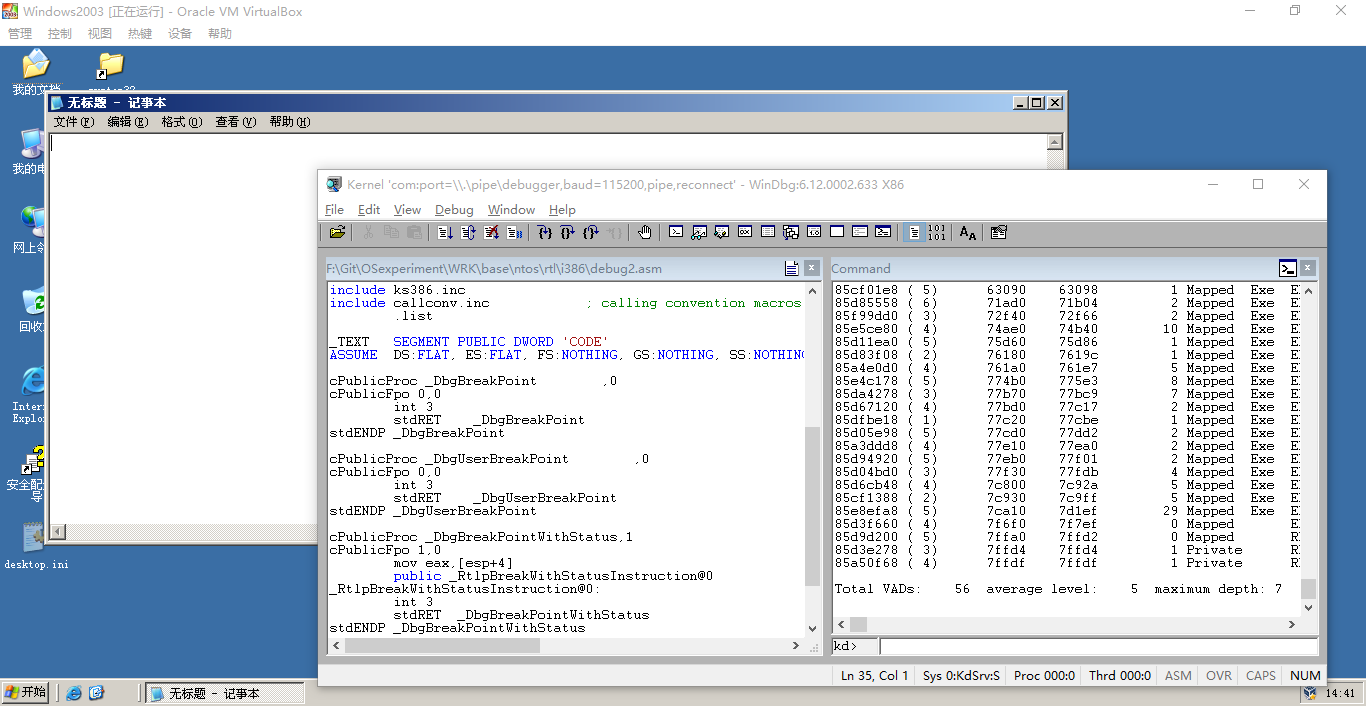
\includegraphics[width=\textwidth]{images/vad4notepad.png}
            \caption{替换内核后运行系统并查看进程的VAD树}
            \label{fig:vad4notepad}
        \end{figure}
        
        使用红黑树实现的VAD树在Windows Server 2003中运行正常。
    
    \section{实验总结}
    
    
    \bibliographystyle{plain}
    \bibliography{ref.bib}
\end{document} 